% Chapter 11

\chapter{Comparación Modelo de la ANN} % Write in your own chapter title
\label{Chapter12}
\lhead{Capítulo 12. \emph{Comparación ANN}} % Write in your own chapter

En este capítulo se analizará comparativamente los niveles de detección entre un modelo de Red Neuronal Artificial usando las herramientas de Matlab (nntool) y el modelo en hardware propuesto en este documento en el Capítulo \ref{Chapter6}, figura \ref{fig:MLP}. El objetivo es demostrar que el modelo propuesto es válido y puede ser implementado a nivel de hardware directamente. Para esto se eligió mostrar la detección del modelo de la red en punto fijo usando el entrenamiento de Matlab con especificaciones iguales a las del modelo Hardware propuesto, por otra parte se usó el entrenamiento directamente sobre el modelo hardware usando C/C++.

\begin{figure}[H]
	\centering
		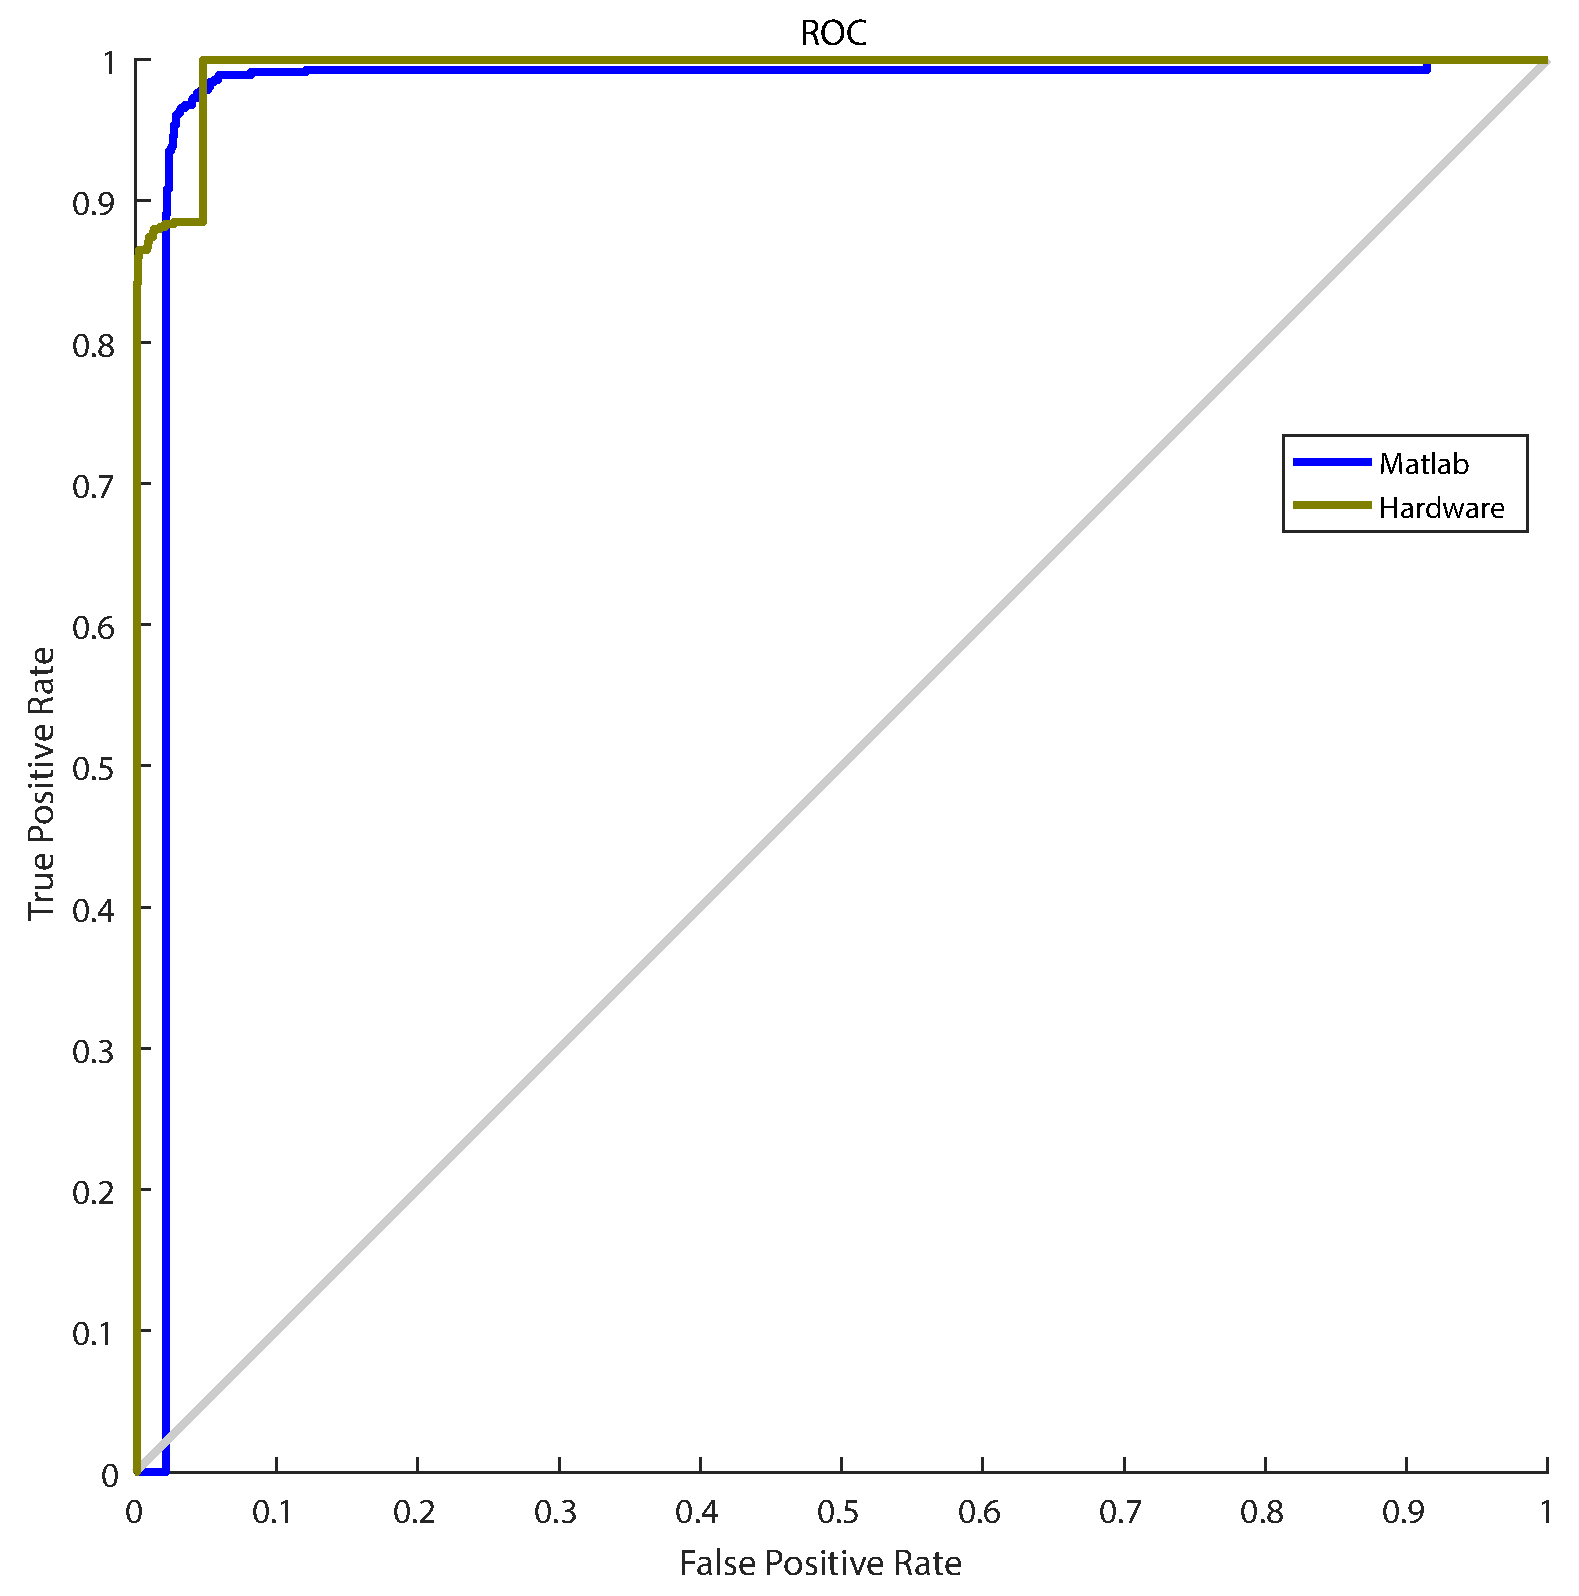
\includegraphics[scale=0.35]{./Figures/ROCANN}
	\caption{Curva ROC de detección}
	\label{fig:ROC}
\end{figure}

 La Figura \ref{fig:ROC} muestra la curva ROC o Receiver Operating Characteristic por sus siglas en inglés, esta gráfica lo que muestra es la calidad del clasificador al discriminar entre un valor de detección positivo y otro negativo basado en el conjunto de datos de entrenamiento. Particularmente una curva ROC muestra lo siguiente según su forma \citep{ROCCurve}:
 
 \begin{itemize}
     \item Se muestra el balance entre la sensibilidad (eje vertical) y la especificidad (eje horizontal), donde un incremento en la sensibilidad va acompañado de un detrimento de la especificadad.
     \item Entre más cerca la curva esté al eje vertical izquierdo y al eje horizontal superior más efectivo es el clasificador.
     \item Entre más cerca esté la curva a la diagonal menos efectivo es el clasificador.
 \end{itemize}
 
 En esta gráfica lo que vemos es que el clasificador tanto en software como en hardware funciona pero debido al entrenamiento presenta algunas detecciones falsas, esto mayoritariamente se debe a las fluctuaciones generadas por el transitorio entre los estados de inundación y sequía propios del conjunto de datos, generando falsos positivos y/o negativos. Esto es posible corregirlo ajustando los parámetros del entrenamiento a tal punto que las fluctuaciones en la detección sean menos notorias, pero particularmente para este problema las transiciones seguirán presentes. Corregir los estados de detección erroneo causados por el entrenamiento y conjunto de datos puede ser corregido ajustando la salida de la RNA con un circuito de retraso que pueda interpretar los rápidos cambios de estado, suavizando la salida de la RNA de tal forma que no se vea afectada la medición final.


Tras analizar ambas redes como clasificador, se hace necesario analizar punto a punto la señal con tal de determinar que efectivamente ambos modelos están entregando punto a punto una equivalencia para el conjunto de datos entregado. Para ello se eligió calcular el indice de correlación y la correlación cruzada. En el primer caso, el índice de correlación es de $0.9329$, siendo un valor de $1$ una perfecta relación positiva entre dos señales \citep{correlation2,correlation}. La Figura \ref{fig:xcorr} muestra la correlación cruzada entre las señales provenientes del modelo de Matlab y el calculado con el entrenamiento sobre el hardware. Se ve claramente que, la forma triangular según la teoría sugiere que se trata de una correlación entre dos señales muy similares entre si, confirmando que el entrenamiento y la detección de ambas redes es equivalente.

\begin{figure}[H]
	\centering
		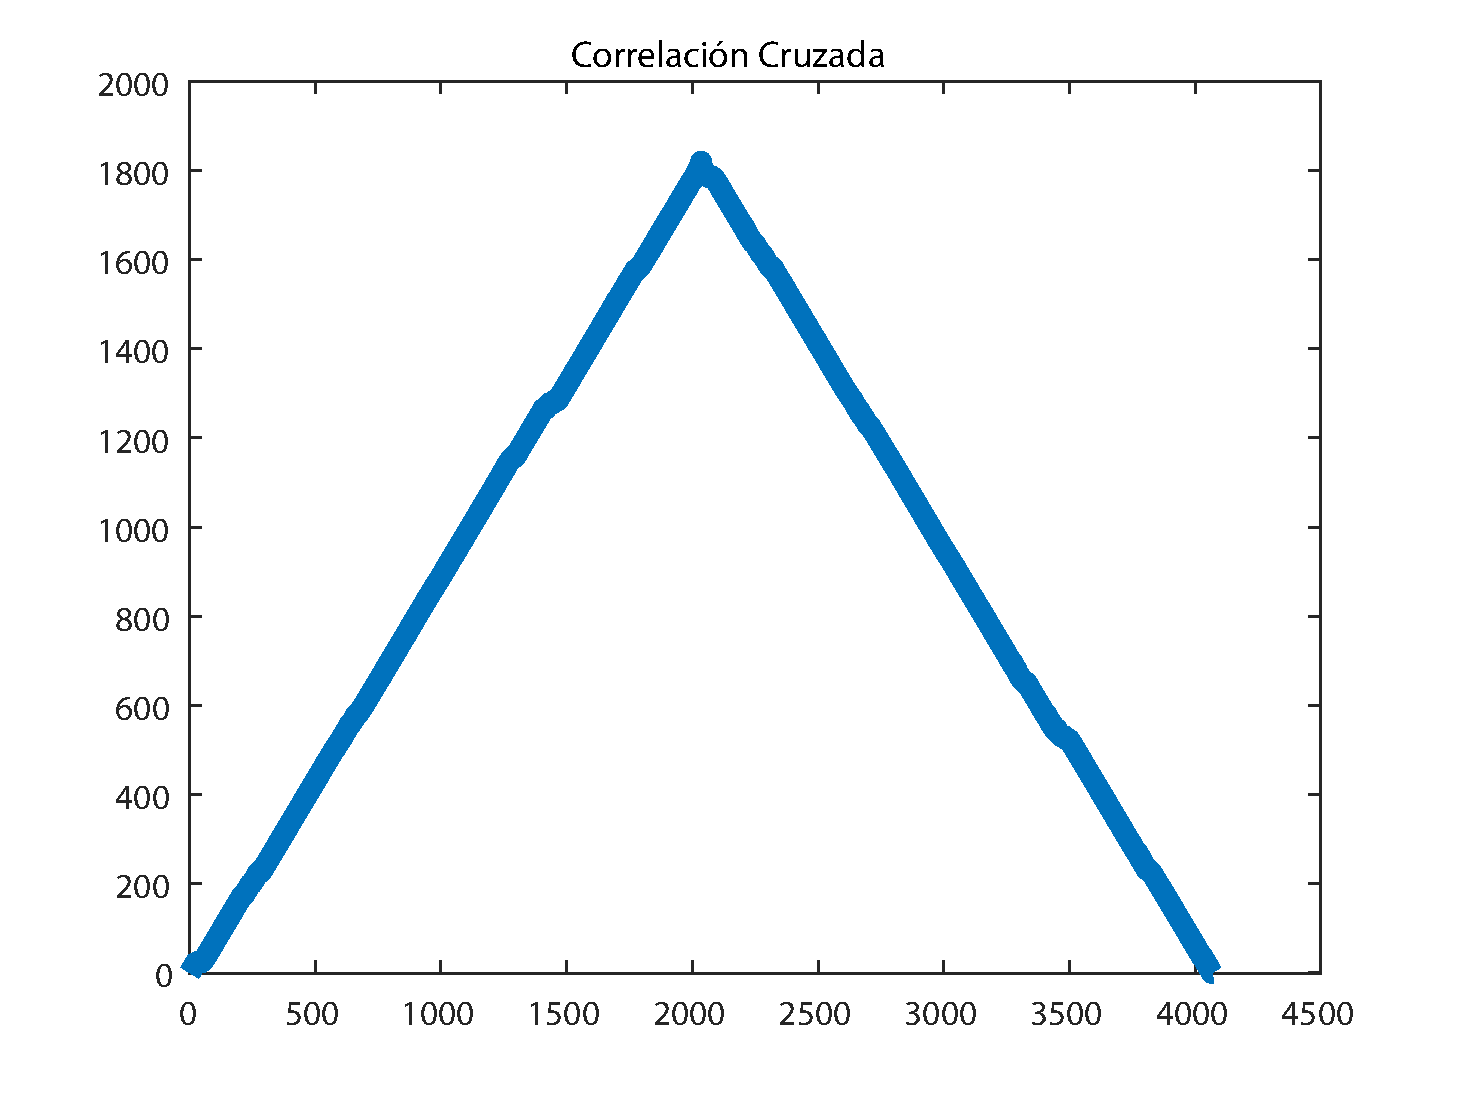
\includegraphics[scale=0.6]{./Figures/xcorrANN}
	\caption{Correlación cruzada entre modelos}
	\label{fig:xcorr}
\end{figure}

Con estos datos, es posible determinar que la implementación en Hardware es correcta y que funcionalmente se encuentra en capacidad de detectar eficazmente la probabilidad de inundación en comparación con un modelo netamente Software como el propuesto usando las herramientas de Matlab.

Es importante mencionar que el rendimiento de ambas redes, tanto la propuesta usando Matlab, como la desarrollada en Hardware dependende directamente de la calidad del entrenamiento y el set de datos elegido.
%Los resultados de detección para la red neuronal aquí expuestos implican que es posible usar configuraciones de redes neuronales mucho más complejas que en Matlab son muy simples de configurar y que los resultados del entrenamiento puedan ser llevados a la implementación Hardware sin dudas que la variación en la detección cambie drásticamente sin necesidad de implementar complejos algoritmos de entrenamiento usando C/C++ directamente sobre el hardware como aquí se propuso.